%\documentclass[10pt]{article}
%\usepackage[usenames]{color} % Farbunterstützung
%\usepackage{amssymb}	% Mathe
%\usepackage{amsmath} % Mathe
%\usepackage[utf8]{inputenc} % Direkte Eingabe von Umlauten und anderen Diakritika\begin{document}
\section{Programmierprojekt}
\authors{Vincent Meise und Felix Forner}
Einen großen Teil der Kurszeit verbrachten wir mit einer Projektarbeit, die das Schreiben von Programmen in Python zur Lösung graphentheoretischer Probleme umfasste. Dabei gaben verschiedene Texte Denkanstöße und Ideen für die Themenfindung. Besonders war dabei aber, dass keine konkreten Aufgabenstellungen vorgegeben wurden. Stattdessen generierte jede Gruppe selbstständig eine angemessene Aufgabe zu der Thematik des gewünschten Textes. \\
Bei den Problemen war es zuerst erforderlich, sich zu \"uberlegen, wie sie graphentheoretisch dargestellt werden können. Um den Erfolg des Projekts zu sichern, sollten einige Überlegungen in einer Vorbereitsungsphase vor der Implementierung getätigt werden. In diesem Rahmen haben wir zuerst die Ein- und Ausgabe spezifiziert. Au\ss erdem brauchten wir eine Erfolgsmetrik, um zu pr\"ufen, ob das Programm wie gew\"unscht funktioniert. Um Chaos w\"ahrend der Entwicklung zu vermeiden, entwarfen wir einen Entwicklungsplan, der das Problem in einzelne Komponenten unterteilt.
Neben dem folgenden Beispielprojekt wurden in anderen Gruppen verschiedene Anwendungen des Dijkstra-Algorithmus\footnote{Der Dijkstra-Algorithmus bestimmt den kürzesten Weg zu jedem Knoten in einem Graphen ausgehend von einem Startknoten.}, eine graphentheoretische Variante der Kryptographie und weitere Themen behandelt.
%-Problemfindung
%-Zielsetzung
%-Erfolgsmetrik
%-Entwicklungsplan, Meilensteine, Evaluation
\subsection{Beispielprojekt}
\subsubsection{Aufgabe} Es soll ein Algorithmus programmiert werden, der pr\"uft, ob zwei eingegebene Graphen isomorph sind oder nicht und entsprechend einen der Wahrheitswerte {\glqq True\grqq} oder {\glqq False\grqq} ausgibt.
\subsubsection{Umsetzung} %Es werden zun\"achst die Anzahl der Knoten und Kanten verglichen. Dann werden die Grade der Knoten bestimmt und es wird gepr\"uft, ob es in beiden Graphen die gleiche Anzahl an Knoten mit den gleichen Grade gibt.
Der erste Ansatz war, ein Programm zu schreiben, das das Problem in polynomieller Laufzeit l\"ost.
W\"ahrenddessen haben wir herausgefunden, dass bisher nur Algorithmen bekannt sind, die das Problem in nicht-polynomieller Zeit l\"osen. Deshalb verfolgten wir die Strategie, die eingegebenen Graphen auf bestimmte Eigenschaften zu pr\"ufen und zu vergleichen. Zu diesen Eigenschaften z\"ahlen die Anzahl der Knoten und Kanten, der Grad der Knoten, Grade von Nachbarknoten, Kreise und L\"angen von k\"urzesten Wegen im Graphen. \\
Wenn die Graphen isomorph sind, kann man mit Hilfe der zuvor genannten Eigenschaften jedem Knoten des einen Graphen einen des anderen Graphen zuordnen. Diese Zuordnung ist nicht zwingend eindeutig, weshalb es nötig sein kann, mehrere Zuordnungen zu testen, bis eine geeignete gefunden ist. Bei isomorphen Graphen gibt es eine solche Zuordnung, bei anderen Graphen nicht. Wenn die Werte nicht zueinander passen, sind die Graphen nicht isomorph. Da der Algorithmus nicht alle möglichen Zuordnungen testet, können einige Eingabegraphen nicht absolut sicher als isomorph identifiziert werden. Der Algorithmus findet lediglich kein Kriterium, das einen Isomorpismus ausschließt. Ein Beispiel solcher zweier Graphen sind $G_1$ aus Abb. \ref{g1} und $G_2$ aus Abb. \ref{g2}.\\
\begin{figure}
\centering
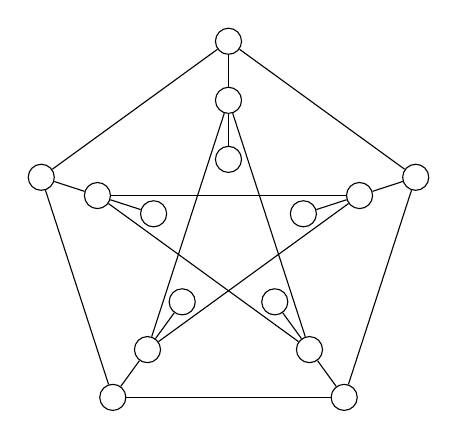
\begin{tikzpicture}
\centering
\node[circle,draw](1) at (18.0:2.5){};
\node[circle,draw](2) at (90.0:2.5){};
\node[circle,draw](3) at (162.0:2.5){};
\node[circle,draw](4) at (234.0:2.5){};
\node[circle,draw](5) at (306.0:2.5){};
\node[circle,draw](6) at (18.0:1.75){};
\node[circle,draw](7) at (90.0:1.75){};
\node[circle,draw](8) at (162.0:1.75){};
\node[circle,draw](9) at (234.0:1.75){};
\node[circle,draw](10) at (306.0:1.75){};
\node[circle,draw](11) at (18.0:1){};
\node[circle,draw](12) at (90.0:1){};
\node[circle,draw](13) at (162.0:1){};
\node[circle,draw](14) at (234.0:1){};
\node[circle,draw](15) at (306.0:1){};
\draw (2)--(1);
\draw (1)--(6);
\draw (2)--(7);
\draw (3)--(8);
\draw (4)--(9);
\draw (5)--(10);
\draw (2)--(3);
\draw (4)--(3);
\draw (5)--(4);
%\draw (6)--(7);
%\draw (7)--(8);
%\draw (8)--(9);
%\draw (9)--(10);
%\draw (6)--(10);
\draw (1)--(5);
\draw (6)--(11);
\draw (7)--(12);
\draw (8)--(13);
\draw (9)--(14);
\draw (10)--(15);
\draw (6)--(8);
\draw (7)--(9);
\draw (8)--(10);
\draw (9)--(6);
\draw (10)--(7);
\end{tikzpicture}
\caption{Graph $G_{1}$}
\label{g1}
\end{figure}\\
$G_{1}$ ist nicht zu $G_{2}$ isomorph. Es ist aber m\"oglich, die Knoten des einen Graphen bijektiv denen des anderen Graphen zuzuordnen, sodass die Grade der Knoten, Nachbarknoten, Nachbarnachbarknoten und Nachbar\ldots nachbarknoten f\"ur jeden Knoten von $G_{1}$ mit dem zugeordneten Knoten von $G_{2}$ \"ubereinstimmen.\\
\begin{figure}
\centering
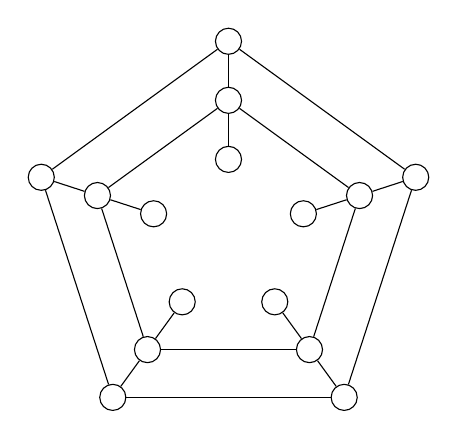
\begin{tikzpicture}
\centering
\node[circle,draw](1) at (18.0:2.5){};
\node[circle,draw](2) at (90.0:2.5){};
\node[circle,draw](3) at (162.0:2.5){};
\node[circle,draw](4) at (234.0:2.5){};
\node[circle,draw](5) at (306.0:2.5){};
\node[circle,draw](6) at (18.0:1.75){};
\node[circle,draw](7) at (90.0:1.75){};
\node[circle,draw](8) at (162.0:1.75){};
\node[circle,draw](9) at (234.0:1.75){};
\node[circle,draw](10) at (306.0:1.75){};
\node[circle,draw](11) at (18.0:1){};
\node[circle,draw](12) at (90.0:1){};
\node[circle,draw](13) at (162.0:1){};
\node[circle,draw](14) at (234.0:1){};
\node[circle,draw](15) at (306.0:1){};
\draw (2)--(1);
\draw (1)--(6);
\draw (2)--(7);
\draw (3)--(8);
\draw (4)--(9);
\draw (5)--(10);
\draw (2)--(3);
\draw (4)--(3);
\draw (5)--(4);
\draw (6)--(7);
\draw (7)--(8);
\draw (8)--(9);
\draw (9)--(10);
\draw (6)--(10);
\draw (1)--(5);
\draw (6)--(11);
\draw (7)--(12);
\draw (8)--(13);
\draw (9)--(14);
\draw (10)--(15);
%\draw (6)--(8);
%\draw (7)--(9);
%\draw (8)--(10);
%\draw (9)--(6);
%\draw (10)--(7);
\end{tikzpicture}
\caption{Graph $G_{2}$}
\label{g2}
\end{figure}\\
\subsubsection{Fazit}
Das Problem hat sich während des Entwicklungsprozesses als schwerer als erwartet herausgestellt, weshalb der Entwicklungsplan weiterentwickelt und abge{\"a}ndert werden musste. Trotzdem ist der finale Algorithmus zufriedenstellend, da die Laufzeit f{\"u}r die meisten Eingabegraphen kurz ist.
